\subsection{HTB04 - Omni}

    \subsubsection{Escaneo}
        \large{Como primera etapa de la Prueba de Penetración realizamos un escaneo de puertos abiertos en la máquina víctima con la herramienta "Nmap", donde se encuentraron 2 de ellos, uno el servicio 'msrpc' y ek otro con el servicio 'upnp'.}
        \par
        \begin{figure}[h!]
            \centering
            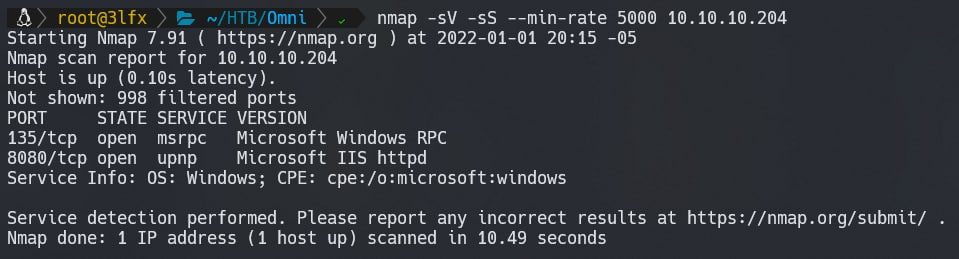
\includegraphics[width=0.99\textwidth]{informe4/imagenes/omni/01_escaneo.png}
            \caption{Escaneo de puertos Omni} 
        \end{figure}  

    \subsubsection{Análisis de Vulnerabilidades}

    \subsubsection{Explotación}

    \subsubsection{Escalamiento de Privilegios}

    \subsubsection{Post-Explotación}

    \subsubsection{Recomendaciones de Mitigación}